\section{RHUL SPA Anritsu}
The SPA has important parameters:
\begin{itemize}
\item \textbf{Span} - the total range of frequencies to analyse;
\item \textbf{RadioBandwidth (RBW)}  - the bandwidth of the filter  which operates on the down-shifted signal.  If it is
  large then  measurements are quick, since  you measre the power  over a wide range.  If it is small,  measurements are
  accurate,  since you  average over  a small  number of  frequencies  at a  single time.  Think of  it as  a window  of
  integration;
\item \textbf{VideoBandwidth (VBW)}  - the bandwidth of  the final filter, which  can remove noise from  the system. The
  signal that  makes it through  the RadioBandwidth filter  can be analysed  with a further  filter, which will  pick up
  random fluctuations and average them out;
\item \textbf{\red{Make sure that TIMESPAN is automatic!} Or else the SPA will not used the parameters set.}
\end{itemize}

In total, the time taken will be (provided that VB is less than RBW):
\[
  t = \frac{\text{SPAN}}{\text{RBW}\times\text{VB}}.
\]


\paragraph{Spectrum analyser} simply  takes the power at different  frequencies. There is no phase  correlation with the
signal that is fed into the system originally
\begin{figure}[h]
  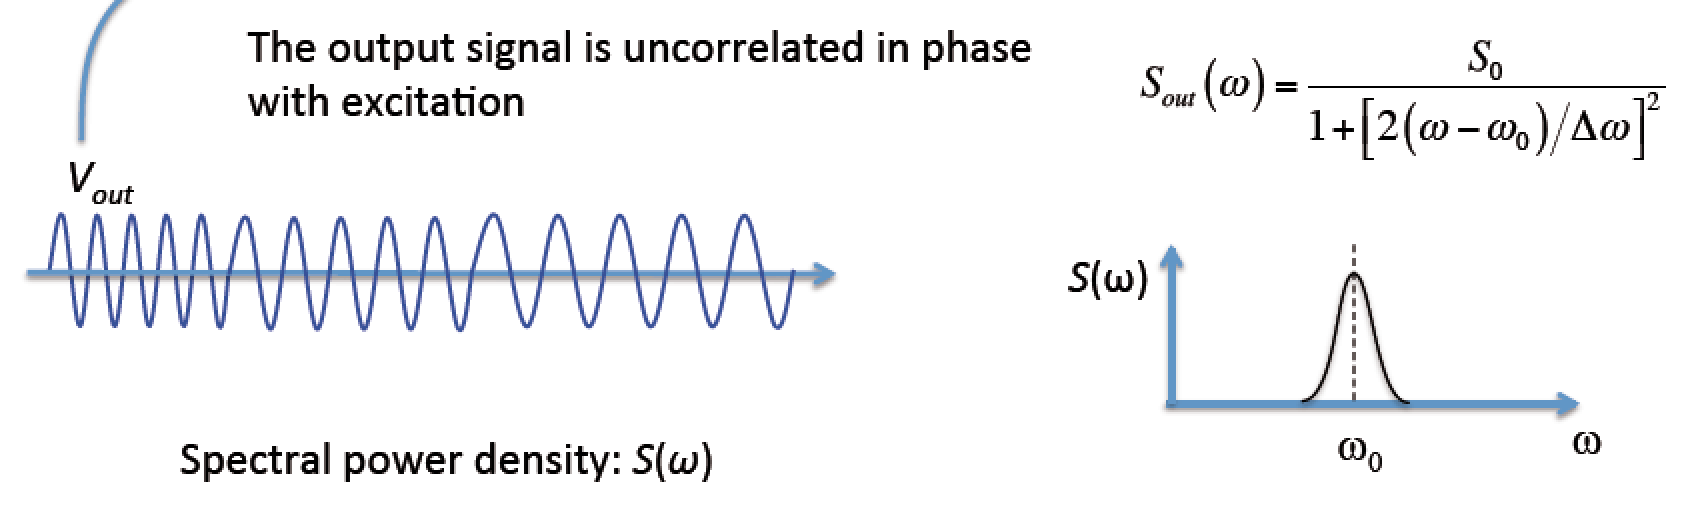
\includegraphics[height=4cm]{spec}
\end{figure}
\newpage
